%%%%%%%% COMPSCI 2430 MIDTERM REPORT (ICML 2025 template)%%%%%%%%
%%%%%%%%%%%%%%%%%%%%%%%%%%%%%%%%%%%%%%%%%%%%%%%%%%%%%%%%%%%%%%%%%%%%%%%%%%%%

\documentclass{article}

\usepackage{microtype}
\usepackage{graphicx}
\usepackage{subfigure}
\usepackage{booktabs}
\usepackage{hyperref}

\newcommand{\theHalgorithm}{\arabic{algorithm}}

% [accepted] prints author names (course report, not a blind review).
\usepackage[accepted]{icml2025}

\usepackage{amsmath}
\usepackage{amssymb}
\usepackage{mathtools}
\usepackage[capitalize,noabbrev]{cleveref}
\usepackage{xcolor}

\icmltitlerunning{How Much KV Cache Can Speculative Decoding Offload?}

\begin{document}

\twocolumn[
\icmltitle{How Much KV Cache Can Speculative Decoding Offload on a Grace Hopper Superchip?}

% Empty affiliation labels: no superscript numbers after the names.
\begin{icmlauthorlist}
\icmlauthor{Ellie Vitanov}{}
\icmlauthor{Mary Guan}{}
\icmlauthor{Wency Suo}{}
\end{icmlauthorlist}

\icmlkeywords{Speculative decoding, KV cache offloading, Grace Hopper, NVLink-C2C}

\vskip 0.3in
]

%==========================================================================
\begin{abstract}
Speculative decoding speeds up text generation by checking several drafted tokens in each pass of the large model, but every pass must still read the model's entire KV cache, which at long context competes with the weights for GPU memory. Offloading part of the cache to CPU memory frees GPU memory at the cost of transfers over a slower link. We ask how much of the cache speculative decoding can offload while staying as fast as ordinary decoding with the whole cache on the GPU. On an NVIDIA L40S over PCIe, speculation tolerates offloading far better than ordinary decoding: at 8K context it stays within 5\% of that baseline with 58\% of the cache offloaded, versus 3\% for ordinary decoding, and at 16K it overtakes ordinary decoding once 20\% is offloaded. A per-layer pipeline model with no fitted parameters predicts these measurements within 3.2\% on average and predicts that at a Grace Hopper superchip's bandwidth ratio offloading one sequence's cache is nearly free. We then measured on a GH200. For speculation the prediction holds: offloading the entire cache costs 3\% per token at 16K. For ordinary decoding it does not: full offload costs 52\%, because on this hardware the decode step is bound by CPU-side kernel launches rather than by GPU work, which the model does not represent. A DirectKV-style zero-copy variant, in which the attention kernel reads the cache in place over NVLink-C2C at 95\% of copy-engine bandwidth, wins ordinary decoding at every context but loses speculation at 16K and above because the library's attention path re-reads the cache four times. We identify 19\,ms of avoidable GPU work per verification step, validate fixes on a second GPU, and lay out the GPU-bound re-measurement that will settle the comparison.
\end{abstract}

%==========================================================================
\section{Introduction}
\label{sec:intro}

Speculative decoding~\citep{leviathan2023fast,chen2023accelerating} works like branch prediction for text generation: a small drafter guesses the next several tokens, the large target model checks all of them in one forward pass, and the correct prefix is kept while the rest is squashed. With block-diffusion drafters such as DFlash~\citep{chen2026dflash}, each verification step commits $\tau$ tokens on average. Every step must still read the target's entire KV cache, the stored keys and values of all previous tokens. For Qwen3-8B~\citep{qwen3} this is 144\,KiB per token, or 2.4\,GB for a single 16K-token sequence; at long context and high concurrency the cache, not the weights, fills GPU memory.

Offloading part of the cache to CPU memory frees GPU memory, but places the offloaded bytes behind a slower link. Offloading systems for ordinary decoding were first built for PCIe~\citep{sheng2023flexgen,jiang2025neo}; on GH200, Pie offloads only as much as transfers can hide behind computation~\citep{xu2024pie}, and DirectKV makes the transfers themselves cheaper~\citep{luo2026directkv}. What matters for offloading is the ratio of link to GPU memory bandwidth: 1/64 for our PCIe-attached L40S (13.5\,GB/s against 864\,GB/s), versus 1/10 on a GH200, where NVLink-C2C moves 415.7\,GB/s from pinned host memory into a GPU with roughly 4\,TB/s of HBM~\citep{fusco2024gh200}.

\textbf{Speculation changes the offloading budget.} The cost of streaming offloaded KV is paid once per verification step but shared by the $\tau$ tokens that step commits, and a verification step computes longer per layer, leaving more time to hide transfers. We ask: \emph{how much of the KV cache can speculative decoding offload while remaining as fast per token as ordinary decoding with the whole cache on the GPU, and how does the answer change on a Grace Hopper superchip?}

\begin{table}[t]
\caption{Where KV-cache offloading has been studied.}
\label{tab:gap}
\vskip 0.1in
\begin{center}
\begin{small}
\begin{tabular}{@{}lll@{}}
\toprule
 & Ordinary decoding & Speculative decoding \\
\midrule
PCIe GPU & FlexGen, Neo & TriForce, SpecStream, \\
         &              & Adaptive DHiSparse \\
GH200    & Pie, DirectKV & \textbf{This work} \\
\bottomrule
\end{tabular}
\end{small}
\end{center}
\vskip -0.1in
\end{table}

\textbf{Novelty.} \Cref{tab:gap} places this question among prior work. Speculative decoding combined with KV offloading has so far been studied only on PCIe-attached GPUs~\citep{sun2024triforce,li2026specstream,alazhar2026dhisparse}, where SpecStream finds that offloaded speculation stays slower than fully GPU-resident speculation on long inputs because of the PCIe link~\citep{li2026specstream}. Offloading on GH200 has been studied only for ordinary decoding~\citep{xu2024pie,luo2026directkv}. MagicDec shows that KV reads are what make speculation pay off at long context, but keeps the cache in GPU memory~\citep{sadhukhan2025magicdec}.

\textbf{Status.} We have implemented a speculation-aware KV manager inside DFlash's generation loop, measured offloading for ordinary and speculative decoding at 8K and 16K context on an L40S, and built a parameter-free pipeline model that matches those measurements (\cref{fig:budget}). We have since rerun the same sweep on a GH200 (\cref{fig:gh200}), added and measured a zero-copy arm, profiled where each step's time goes, and tested a first eviction policy (\cref{sec:gh200}).

%==========================================================================
\section{Challenges}
\label{sec:challenges}

\textbf{Hiding versus paying for transfers.} Offloaded KV must arrive before the layer that needs it. Transfers hidden behind computation are free; anything beyond that adds to every step, and its cost per token depends on the link and on $\tau$.

\textbf{The step is not GPU-bound.} DFlash's research loop handles one sequence at a time in eager PyTorch: about 2{,}250 kernel launches per decoding step, each costing 15--20\,$\mu$s of CPU time, while the GPU work for one token is 10\,ms. On the GH200 an ordinary step therefore takes 48\,ms of which the GPU is busy 21\%. Transfers that ``hide'' may be hiding behind Python rather than behind computation, and a model that assumes a GPU-bound step mispredicts.

\textbf{Measurement fidelity.} The verification step grows with context because Transformers' attention path materialises a four-fold expanded copy of the cache for multi-token attention; with the cache in host memory that copy is what crosses the link. The stock cache also appends to a growing tensor every step, which costs 13\,ms of CPU time per step on the GH200, so the all-resident configuration of our own cache is the fair baseline. Acceptance varies by prompt, so we use fixed prompts, decode greedily, and check that offloaded and all-GPU runs emit identical tokens.

%==========================================================================
\section{Design}
\label{sec:design}

\textbf{Speculation-aware KV split.} Following SpecStream's commit-aware tiering~\citep{li2026specstream}, verified history lives in pinned CPU memory, while recent tokens and the current speculative block stay on the GPU, so rejected guesses are discarded without crossing the link. A knob keeps the first $R$ of the model's $L=36$ layers entirely on the GPU, which sets the offloaded fraction $f$. Offloaded layers are fetched one at a time on a separate copy stream into a ring of two staging buffers, so a layer's fetch can overlap computation of the layers before it. The manager plugs into DFlash's Transformers implementation~\citep{wolf2020transformers} without modifying DFlash.

\textbf{Pipeline model.} Offloading cost comes down to two per-layer times: $t$, the time to fetch one layer's KV over the link, and $c$, the time the GPU spends computing one layer,
\begin{equation}
t = \frac{nb}{L\,B_\text{link}}, \qquad c = \frac{T}{L}.
\label{eq:times}
\end{equation}
Here $nb$ is one sequence's KV cache in bytes ($n$ tokens of $b$ bytes each), so $nb/L$ is one layer's share; $B_\text{link}$ is the host-to-GPU bandwidth; and $T$ is the measured time of one decoding step with the whole cache on the GPU, so $T/L$ is one layer's share. Fetching and computing overlap like an assembly line: while the GPU computes one layer, the link delivers the next. If delivery is slower ($t > c$), the GPU waits and each offloaded layer adds about $t - c$ to the step; if delivery is faster ($t \le c$), offloading is nearly free. Speculation helps in two ways: each layer processes a whole block of guesses, which raises $c$, and each step produces $\tau$ tokens on average (the accepted guesses plus one), so its cost is shared across them; ordinary decoding has $\tau = 1$. We simulate this pipeline exactly for each prompt, including that only two layers can be fetched ahead (one per staging buffer), and report time per token as the simulated step time divided by $\tau$. The model has no fitted parameters: its inputs are the measured all-GPU step time and $\tau$ for each prompt, plus $B_\text{link}$ from a separate bandwidth benchmark. For the GH200 projection we change only $B_\text{link}$, to GH200's link-to-memory ratio (415.7\,GB/s over about 4\,TB/s~\citep{fusco2024gh200}) applied to the L40S's 864\,GB/s memory, about 90\,GB/s.

\textbf{Zero-copy branch.} DirectKV-style zero-copy \citep{luo2026directkv} has the attention kernel read offloaded KV directly from host memory. This removes the staging buffers but also the lookahead: a layer's KV moves only during that layer's attention call. We model the time of an offloaded layer as
\begin{equation}
c_{\text{zc}} = c_{\text{other}} + \max\!\left(c_{\text{attn}},\, \frac{t}{\eta}\right),
\label{eq:zerocopy}
\end{equation}
where $c_{\text{attn}}$ and $c_{\text{other}}$ split each measured layer time between attention and everything else, and $\eta$ is the fraction of link bandwidth that loads issued from inside a kernel achieve. $\eta$ was the one parameter we assumed; on the GH200 we measured it (\cref{sec:gh200}) and implemented the branch as a fourth arm of the manager, which keeps offloaded layers in GPU-mapped pinned memory and hands the attention call a view of it.

\textbf{Offload budget.} We define a mode's budget as the largest offloaded fraction at which its time per token stays within 5\% of ordinary decoding with the whole cache on the GPU.

%==========================================================================
\section{L40S Measurements and Model}
\label{sec:eval}

\textbf{Setup.} One NVIDIA L40S (48\,GB GDDR6, PCIe Gen4) on an AWS g6e.2xlarge instance with NVIDIA driver 595.112.07 and CUDA 13.2; PyTorch 2.13 and Transformers 5.15; Qwen3-8B with the \texttt{z-lab/\allowbreak Qwen3-8B-\allowbreak DFlash-b16} drafter (16-token blocks) in bf16; greedy decoding; one sequence at a time; 256 generated tokens per prompt. We use six prompts each from SPEED-Bench's 8K and 16K throughput splits~\citep{abramovich2026speedbench} and sweep $R \in \{36, 32, 27, 18, 9, 0\}$, i.e., offloaded fractions from 0 to 0.99. Ordinary decoding runs the same loop with a block size of 1.

\textbf{Correctness.} All 144 offloaded runs emit token-for-token identical outputs to the corresponding all-GPU runs, consistent with our earlier CPU tests on small random models.

\begin{figure*}[t]
\vskip 0.1in
\begin{center}
\subfigure[8K context]{%
  \IfFileExists{figs/fig_offload_budget_8k.png}{%
    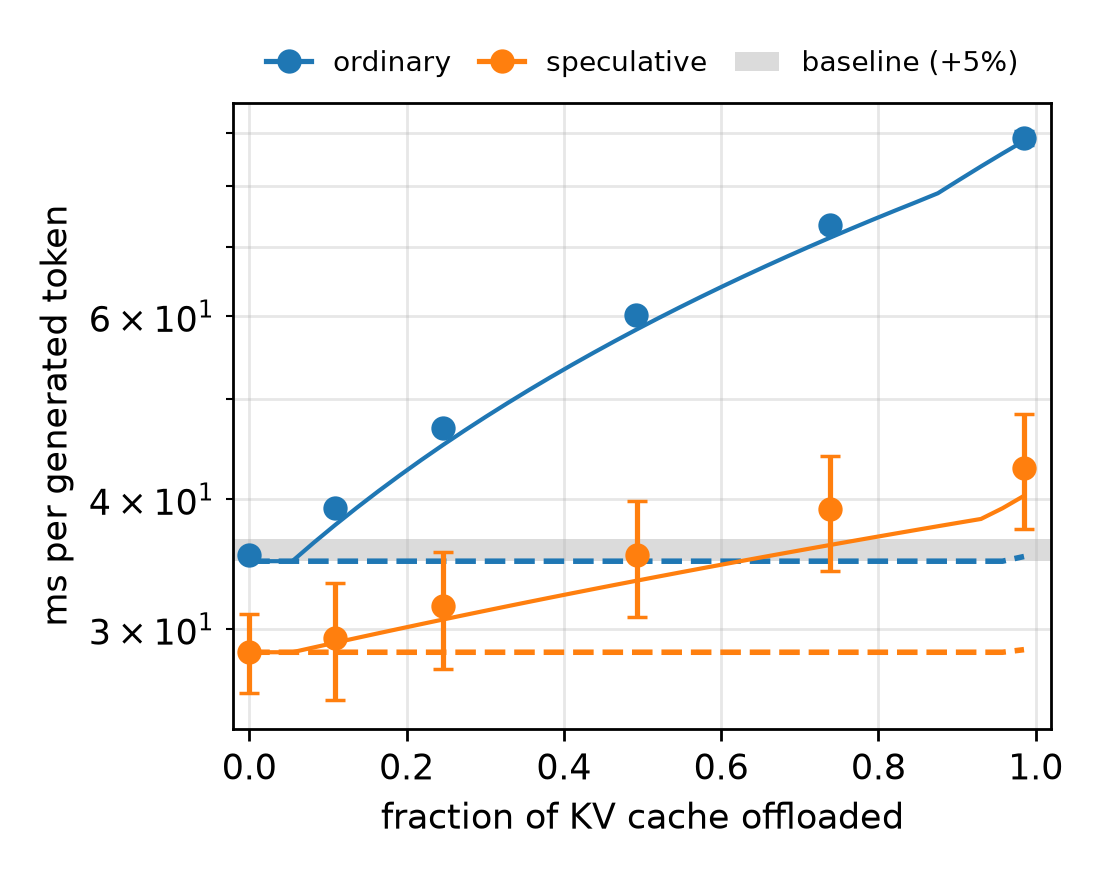
\includegraphics[width=0.48\textwidth]{figs/fig_offload_budget_8k.png}}{%
    \fbox{\parbox[c][5cm][c]{0.46\textwidth}{\centering
    \fillin{figs/fig\_offload\_budget\_8k.png}}}}}
\hfill
\subfigure[16K context]{%
  \IfFileExists{figs/fig_offload_budget_16k.png}{%
    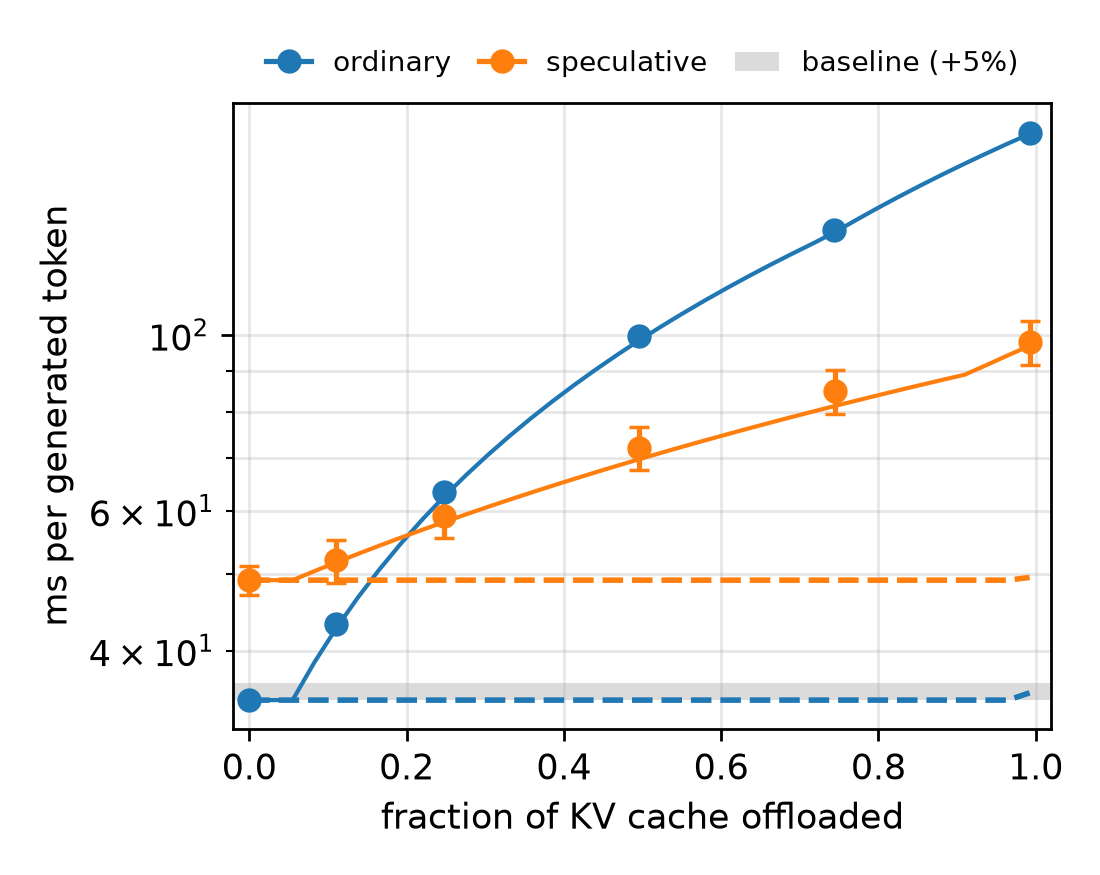
\includegraphics[width=0.48\textwidth]{figs/fig_offload_budget_16k.png}}{%
    \fbox{\parbox[c][5cm][c]{0.46\textwidth}{\centering
    \fillin{figs/fig\_offload\_budget\_16k.png}}}}}
\caption{Time per generated token versus fraction of the KV cache offloaded (Qwen3-8B, one sequence). Points: mean over six prompts measured on the L40S over PCIe (bars: standard error). Solid lines: pipeline model at the measured PCIe bandwidth. Dashed lines: the same model at GH200's link-to-memory ratio; for ordinary decoding it stays at the all-GPU time, so offloading is free there. Gray band: ordinary decoding with nothing offloaded, up to 5\% above it; a curve is within its offload budget while it stays at or below the band. (a)~Speculation stays at or below the band until 58\% of the cache is offloaded; ordinary decoding rises above it immediately. (b)~Speculation starts slower but overtakes ordinary decoding once 20\% is offloaded.}
\label{fig:budget}
\end{center}
\vskip -0.2in
\end{figure*}

\textbf{Speculation weakens at long context in this setup.} On four short GSM8K prompts, speculation accepts about 5.5 tokens per step and runs 4.2$\times$ faster than ordinary decoding. On SPEED-Bench it accepts 2.5 tokens per step at 8K and 1.9 at 16K, and its verification step grows from 63 to 92\,ms, while an ordinary step stays near 35\,ms at every length, which suggests it is dominated by per-step software overhead. With the whole cache on the GPU, speculation is therefore 1.22$\times$ faster than ordinary decoding at 8K but 1.4$\times$ slower at 16K. GSM8K and SPEED-Bench also differ in task type, so we cannot yet attribute the drop in acceptance to context length alone.

\textbf{Speculation tolerates offloading far better.} Over PCIe, fetching one layer's KV takes longer than computing it (\cref{tab:inputs}), so the link sets the pace and ordinary decoding slows down as soon as anything is offloaded (budgets of 0.02--0.03). Speculation stays within 5\% of the ordinary baseline until 58\% of the cache is offloaded at 8K. At 16K it overtakes ordinary decoding at the same offloaded fraction above 0.20, and with the whole cache offloaded it is 1.8$\times$ faster (98 versus 179\,ms per token): a verification step hides more of each fetch behind its longer per-layer computation and shares the rest across $\tau$ tokens.

\begin{table}[t]
\caption{Measured model inputs and results on the L40S (PCIe) and the model's projection to GH200's bandwidth ratio, which changes only the link. Budgets use the 5\% criterion of \cref{sec:design}; ``none'' means already slower with nothing offloaded.}
\label{tab:inputs}
\vskip 0.1in
\begin{center}
\begin{small}
\setlength{\tabcolsep}{3.2pt}
\begin{tabular}{@{}lrrrr@{}}
\toprule
 & \multicolumn{2}{c}{8K context} & \multicolumn{2}{c}{16K context} \\
\cmidrule(lr){2-3}\cmidrule(lr){4-5}
 & PCIe & GH200 & PCIe & GH200 \\
\midrule
Link bandwidth (GB/s)       & 13.5 & 89.8 & 13.5 & 89.8 \\
KV per sequence (GB)        & 1.18 &      & 2.40 &      \\
Fetch per layer $t$ (ms)    & 2.43 & 0.36 & 4.95 & 0.74 \\
Ordinary step $T_N$ (ms)    & 34.9 &      & 34.6 &      \\
Speculative step $T_S$ (ms) & 62.9 &      & 91.6 &      \\
Tokens per step $\tau$      & 2.52 &      & 1.90 &      \\
\midrule
Budget, ordinary            & 0.03 & 0.99 & 0.02 & 0.99 \\
Budget, speculative         & 0.58 & 0.99 & none & none \\
Spec.\ faster above         & 0    & 0    & 0.20 & never \\
\bottomrule
\end{tabular}
\end{small}
\end{center}
\vskip -0.1in
\end{table}


\textbf{The model matches the measurements.} Without fitted parameters, the pipeline model predicts all 24 measured configurations within 3.2\% on average (worst case 7.6\%) and reproduces the 16K crossover at 0.20, which is why we use it for the GH200 projection.

\textbf{At GH200's ratio the model says one sequence offloads for free.} A layer then fetches in 0.4--0.7\,ms, faster than it computes, so both modes should offload nearly the whole cache within 5\% (\cref{fig:budget}, dashed). \Cref{sec:gh200} tests this: it holds for speculation and fails for ordinary decoding.

\textbf{Zero-copy matches copy only when attention takes longer than the read.}
We measured $c_{\text{attn}}$ as the GPU time of each layer's attention module, using CUDA events recorded by forward hooks before and after it, averaged over decode steps on the sweep's prompts. This time covers the Q, K, V and output projections, rotary embedding, cache update, GQA expansion copy and SDPA kernel; we set $c_{\text{other}} = T/L - c_{\text{attn}}$. Qwen3-8B has four query heads per KV head, so each KV byte is read by 4 query rows in an ordinary step and 64 in a 16-token verification step. Copy-based prefetch overlaps a layer's transfer with the previous layer; zero-copy overlaps it only with that layer's attention module. Zero-copy therefore adds no time when $\rho \geq 9.6/\eta$, where $\rho$ is $c_{\text{attn}}$ divided by the time to read the layer's KV from GPU memory and 9.6 is GH200's ratio of memory to link bandwidth. Verification spends 47--60\% of each layer in attention ($\rho \approx 20$) and matches copy for $\eta \geq 0.5$ (\cref{tab:zerocopy}); ordinary decoding spends 31--43\% ($\rho \approx 5$--$8$), and its offload budget falls from 0.99 to 0.04--0.64.

The match depends on our attention path, which builds a GQA-expanded copy of the cache. With a GQA-native kernel, the module would take about as long as reading the projection weights and the KV once, giving $\rho \approx 2$--$4$, so for one sequence zero-copy would add time in both modes. Since attention performs about one floating-point operation per KV byte per query row,
zero-copy would match copy only with about 2{,}400 query rows per KV head (GH200's peak BF16 throughput divided by its link bandwidth), or roughly 40 sequences verifying against one shared prefix. This was the prediction before we could measure in-kernel host reads; \cref{sec:gh200} reports the measurement, which reverses it for ordinary decoding.

\begin{table}[t]
\caption{Offload budget at GH200's bandwidth ratio, from the pipeline model: the largest offloaded fraction within 5\% of ordinary all-GPU decoding. $\eta$ is the assumed fraction of link bandwidth reached by in-kernel loads; --: slower than that baseline even with nothing offloaded.}
\label{tab:zerocopy}
\vskip 0.1in
\begin{center}
\begin{small}
\begin{tabular}{@{}llcccc@{}}
\toprule
& & copy & \multicolumn{3}{c}{zero-copy, $\eta=$} \\
\cmidrule(lr){4-6}
& & & 1.0 & 0.75 & 0.5 \\
\midrule
8K  & ordinary    & 0.99 & 0.64 & 0.24 & 0.11 \\
    & speculative & 0.99 & 0.99 & 0.99 & 0.99 \\
16K & ordinary    & 0.99 & 0.15 & 0.08 & 0.04 \\
    & speculative & --   & --   & --   & --   \\
\bottomrule
\end{tabular}
\end{small}
\end{center}
\vskip -0.1in
\end{table}


%==========================================================================
\section{GH200 Measurements}
\label{sec:gh200}

\textbf{Setup.} One NVIDIA GH200 480\,GB (Lambda; Grace CPU, 96\,GB HBM3, NVLink-C2C), driver 595, CUDA 13; the same software stack, prompts, sweep and decoding settings as \cref{sec:eval}. Pinned host-to-GPU bandwidth measured 341\,GB/s at 1\,GiB (350 peak), and an in-kernel read of GPU-mapped host memory 332\,GB/s, 95\% of the copy engine, so $\eta = 0.95$.

\begin{figure*}[t]
\vskip 0.1in
\begin{center}
\subfigure[8K context]{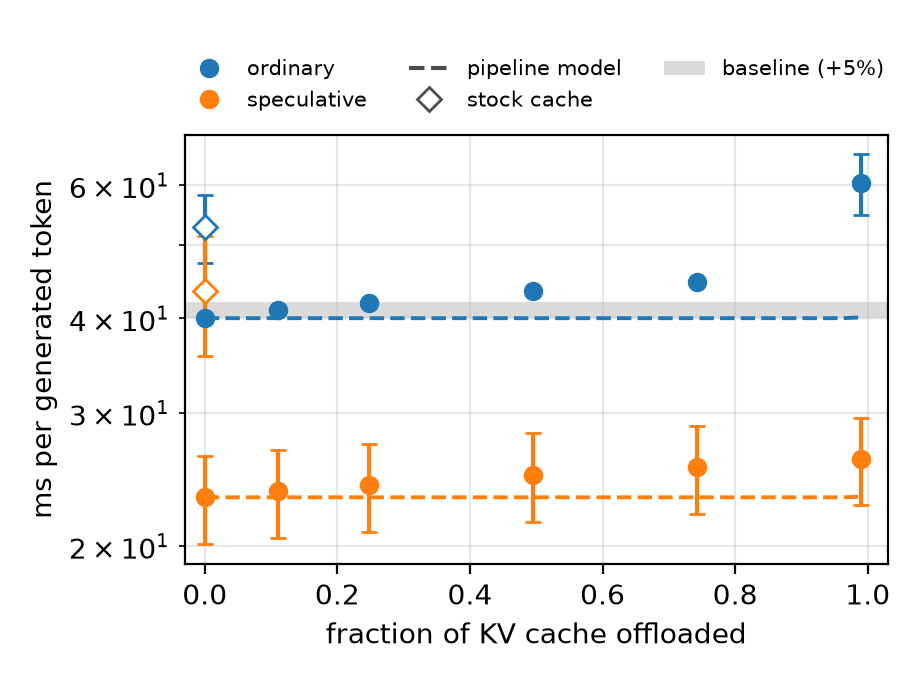
\includegraphics[width=0.48\textwidth]{figs/fig_offload_budget_gh200_8k.png}}
\hfill
\subfigure[16K context]{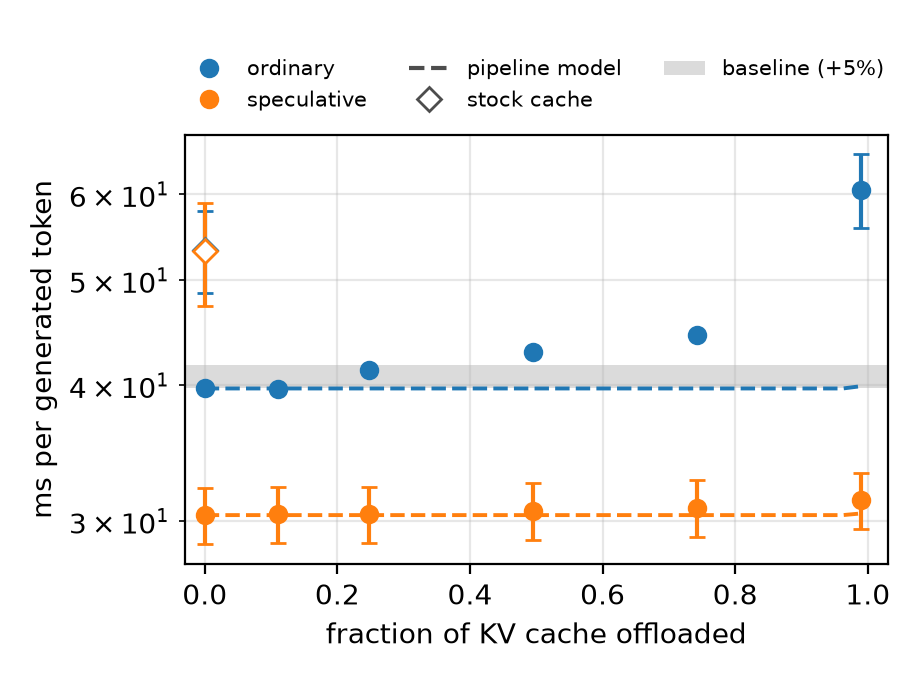
\includegraphics[width=0.48\textwidth]{figs/fig_offload_budget_gh200_16k.png}}
\caption{The same sweep as \cref{fig:budget}, measured on the GH200 (six prompts, bars: standard error). Dashed: the pipeline model of \cref{sec:design} at the measured link bandwidth, with the all-resident configuration of our cache as $T$. Gray band: that baseline plus 5\%. Hollow diamonds: the stock Transformers cache, which is 13\,ms per step slower for CPU-side reasons and was the baseline of \cref{fig:budget}. Speculation is flat across the whole sweep as the model predicts; ordinary decoding rises to $+52\%$ at full offload where the model predicts no change.}
\label{fig:gh200}
\end{center}
\vskip -0.2in
\end{figure*}

\textbf{Speculation offloads for free; ordinary decoding does not.} \Cref{fig:gh200} and \cref{tab:gh200} give the sweep. With the entire cache in host memory a speculative token costs 3\% more at 16K and 12\% at 8K, and the budget is 0.99 at both lengths. Ordinary decoding stays within 5\% only to an offloaded fraction of 0.25 and costs 52\% more at full offload. On the L40S the same offload cost 5$\times$ (ordinary) and 2$\times$ (speculative). With the all-resident cache as baseline, speculation is also faster than ordinary decoding at both lengths (1.73$\times$ at 8K, 1.31$\times$ at 16K); the slowdown at 16K reported in \cref{sec:eval} was a property of the stock cache's CPU overhead, not of speculation.

\begin{table}[t]
\caption{GH200 model inputs and measured results, with the all-resident configuration as baseline. The model predicts both modes offload for free; it misses ordinary decoding by 44\% because the step is CPU-bound (\cref{fig:profile}).}
\label{tab:gh200}
\vskip 0.1in
\begin{center}
\begin{small}
\setlength{\tabcolsep}{4pt}
\resizebox{\columnwidth}{!}{%
\begin{tabular}{@{}lrr@{}}
\toprule
 & 8K & 16K \\
\midrule
Link bandwidth (GB/s)              & 341  & 341 \\
Fetch per layer $t$ (ms)           & 0.10 & 0.20 \\
Ordinary step $T_N$ (ms)           & 40.0 & 39.7 \\
Speculative step $T_S$ (ms)        & 58.0 & 56.4 \\
Tokens per step $\tau$             & 2.50 & 1.86 \\
GPU work per ordinary step (ms)    & --   & 10.2 \\
\midrule
Full offload, ordinary (ms/token)  & 60.3 ($+51\%$) & 60.6 ($+52\%$) \\
Full offload, speculative          & 26.1 ($+12\%$) & 31.4 ($+3\%$) \\
Budget, ordinary / speculative     & 0.25 / 0.99 & 0.25 / 0.99 \\
Model error, ordinary (mean)       & 44\% & 44\% \\
\bottomrule
\end{tabular}}
\end{small}
\end{center}
\vskip -0.1in
\end{table}

\begin{figure*}[t]
\begin{center}
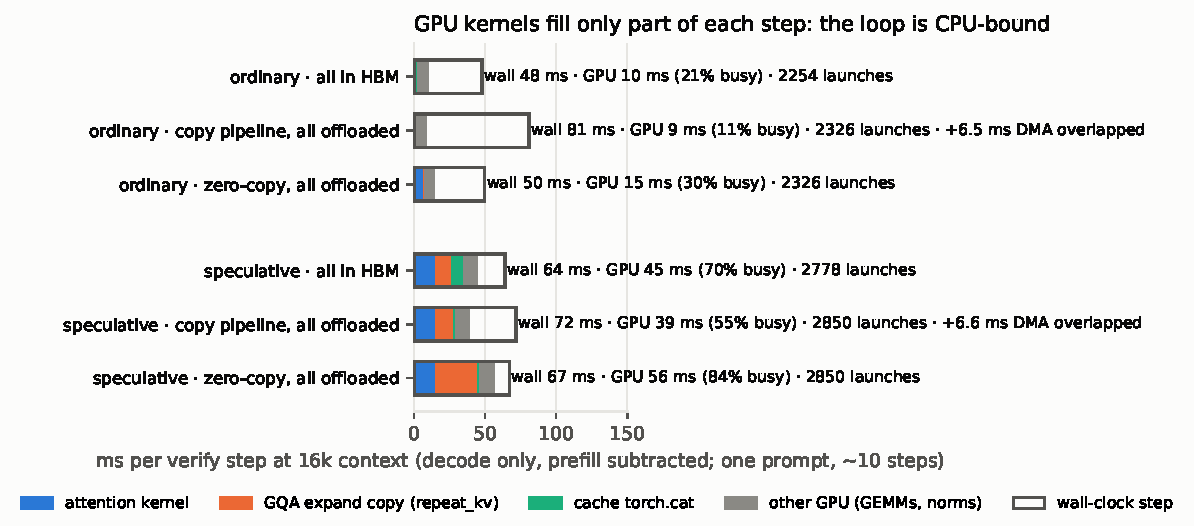
\includegraphics[width=0.92\textwidth]{figs/fig3_where_the_time_goes.pdf}
\caption{Decode-only profile at 16K on the GH200 (one prompt, prefill subtracted). Outline: wall-clock step; fill: GPU kernel time by category. The ordinary step is 10\,ms of GPU work inside 48\,ms; the copy pipeline's 6.5\,ms of DMA overlaps, but its per-layer stream waits on the CPU make it the slowest wall step, while zero-copy's extra in-kernel reads hide in the idle time. Of the verification step's 45 GPU-ms, 19 are the GQA expansion copy and the cache append.}
\label{fig:profile}
\end{center}
\vskip -0.2in
\end{figure*}

\textbf{Why the model misses ordinary decoding.} \Cref{fig:profile} shows a decode-only profile. The ordinary step issues about 2{,}250 kernel launches for 10\,ms of GPU work; the GPU is busy 21\% of the 48\,ms step. In this regime the pipeline's per-layer event waits are paid on the CPU, the scarce resource, which is why the copy pipeline's wall step is the worst of the three arms even though its transfers overlap. Verification is 70\% GPU-bound (45 of 64\,ms), so the model's hiding argument applies there. Refitting the model with a CPU term shows that most of its 44\% error comes from the baseline: the unchanged model with the all-resident step as $T$ has 21\% held-out error, and the CPU term brings it to 12\%.

\begin{figure*}[t]
\begin{center}
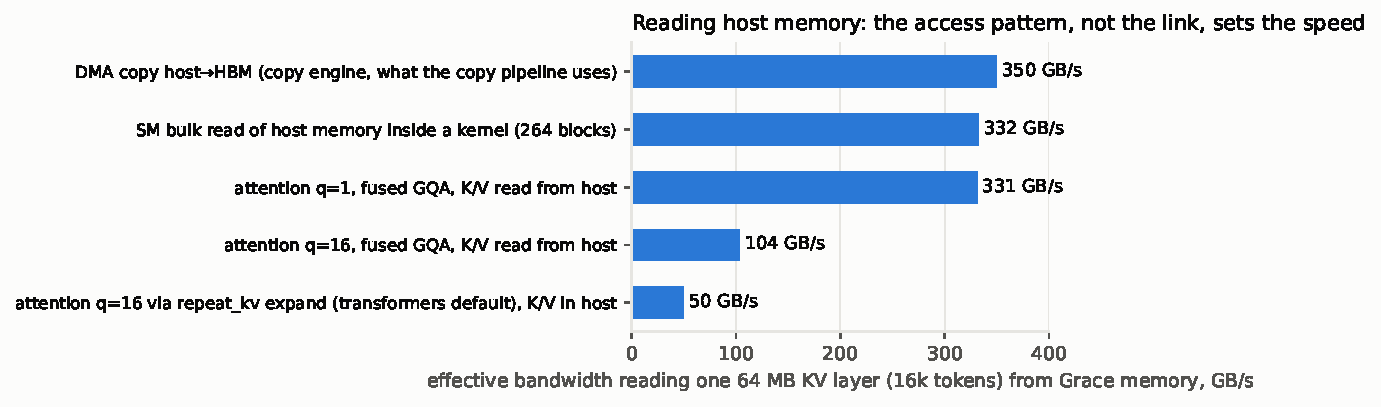
\includegraphics[width=0.92\textwidth]{figs/fig2_host_read_bandwidth_by_access_pattern.pdf}
\caption{Effective bandwidth reading one 64\,MB KV layer (16K tokens) from Grace memory on the GH200, by access pattern. The link is not the limit: in-kernel reads reach 95\% of the copy engine, and single-query attention gets all of it, but the 16-query verification block through Transformers' expansion path gets 50\,GB/s because it reads the cache four times with a strided pattern.}
\label{fig:access}
\end{center}
\vskip -0.2in
\end{figure*}

\begin{figure*}[t]
\vskip 0.1in
\begin{center}
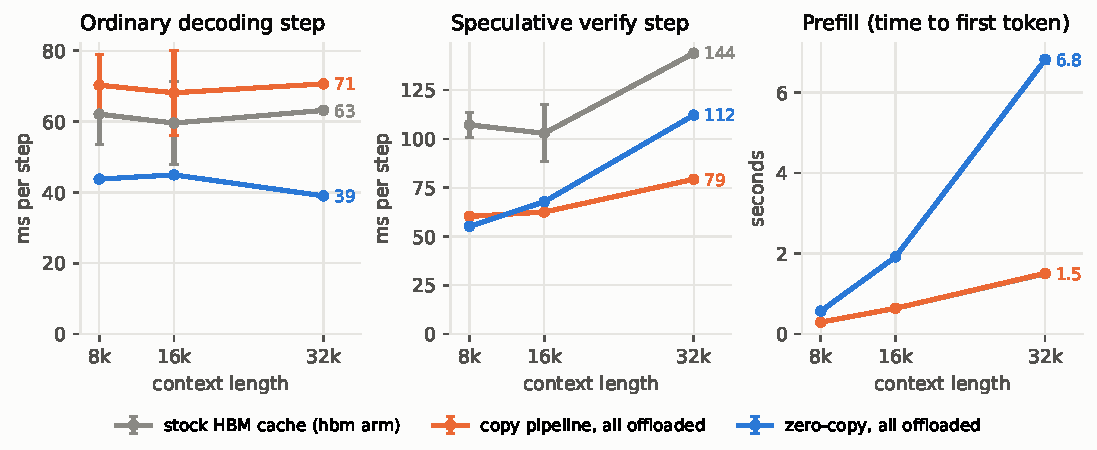
\includegraphics[width=\textwidth]{figs/fig4_zerocopy_vs_copy_vs_context.pdf}
\caption{Zero-copy versus the copy pipeline with the entire cache offloaded, GH200, four prompts (three at 32K). Ordinary decoding: zero-copy wins at every context and its step is flat with length (39\,ms at 32K against 71). Speculation: a tie at 8K, then zero-copy loses 8\% at 16K and 41\% at 32K, the cost of the expansion copy in \cref{fig:access}. Prefill: zero-copy also reads the prompt's cache from host memory, 3--4.5$\times$ slower, which we have since fixed by prefilling in HBM.}
\label{fig:zc}
\end{center}
\vskip -0.2in
\end{figure*}

\textbf{Zero-copy, measured.} \Cref{fig:access} replaces the assumed $\eta$: the GPU reads host memory in place at 332\,GB/s, and single-query attention runs at link speed from host memory (0.20\,ms per layer at 16K). \Cref{fig:zc} gives the end-to-end comparison. Zero-copy wins ordinary decoding everywhere, the opposite of \cref{tab:zerocopy}'s prediction, because the copy pipeline's CPU-side waits cost more than the in-kernel reads it avoids, and those reads hide in the GPU's idle time. For speculation it ties at 8K and loses at 16K and 32K: the profile attributes the loss entirely to the expansion copy reading host memory at about 80\,GB/s (29\,ms per step at 16K), while the attention kernel itself takes the same 15\,ms as from HBM. Once the step is GPU-bound we expect the ordinary-decoding result to flip back, since in-kernel reads cannot overlap the same layer's computation while DMA can; that is the measurement in \cref{sec:plan}.

\textbf{Eviction policy v1.} With the copy pipeline at 16K, keeping the last 2{,}048 tokens of every layer in HBM (448\,MB) gives a 56\,ms verification step, better than keeping half the layers resident (1{,}352\,MB, 58--59\,ms) at a third of the memory, so for speculation a token window is the better eviction unit. For ordinary decoding the opposite holds: resident-first layers (43\,ms) beat resident-last (62) and any token window (62--63), because the pipeline needs the slack of resident layers to prefetch. For zero-copy a token window is a no-op until attention is split between a host prefix and an HBM tail, which we have implemented and tested on the A40 but not yet timed on the GH200.

%==========================================================================
\section{Remaining Challenges and Plan}
\label{sec:plan}

\textbf{Done since the L40S measurements.} The GH200 sweep, the zero-copy arm, the decode-only profile and eviction policy v1 above. From the profile we implemented, with CPU-side tests and a validation pass on a rented A40: an attention path that avoids the GQA expansion (folding the four query heads of each KV head into the query axis so the memory-efficient kernel reads the cache once: $-24\%$ GPU time per verification step, $-33\%$ with a preallocated cache), zero-copy prefill through HBM (time to first token now equal to the copy pipeline's), a KV-stationary Triton kernel that reads host memory once per layer (matches fused attention from HBM at 16K and reads host memory five times more efficiently than either library path), and \texttt{torch.compile} plus CUDA-graph capture of the target forward (kernel launches per step $3\times$ fewer; host launch calls in the target forward from 2{,}072 to 4). All are behind flags that default off, so the numbers in this report reproduce unchanged.

\begin{itemize}
\item \textbf{GPU-bound re-measurement on the GH200} (one session, about 40 GPU-minutes): the four arms at 16K under stock, compiled, graphed and both. This decides whether zero-copy's ordinary-decoding win survives once the step is GPU-bound. Our projection from the profile: ordinary decoding becomes link-bound (full offload $+25\%$ at 16K, $+55\%$ at 32K), speculation stays nearly free, and zero-copy ties the copy pipeline only with the KV-stationary kernel.
\item \textbf{Batches of sequences sharing a prefix.} The manager and DFlash's loop are batch-size one. We will add a shared-prefix segment plus per-request suffixes, read the prefix once per step for all requests in the kernel, and sweep the fan-out at 16K and 32K. This is the regime in which the fetch is paid once and the computation $B$ times.
\item \textbf{Open items from the GH200 run.} Block-size-1 outputs of offloaded arms differ from the stock cache on half the prompts there (a kernel-dispatch difference, not reproduced on the A40); a 40--75\,ms host-side stall appears once mapped pinned memory is allocated in a process and needs a root cause if it shows in per-step timings; the drafter is still eager and now dominates launches at block 16.
\item \textbf{Context versus task.} Separate the effect of context length on acceptance from that of task type, using verification-width traces.
\end{itemize}

\textbf{Timeline.}
Week 8: GPU-bound GH200 session, drafter capture. Weeks 9--10: batched shared-prefix benchmark and kernel, throughput measurements. Week 11: final report and presentation.

\bibliography{references}
\bibliographystyle{icml2025}

\end{document}
